\begin{framed}

Objetivos:
\begin{itemize}
    \item Conocer soluciones de capa límite diferentes a una placa plana. 
\end{itemize}

Contenidos:
\begin{itemize}
    \item Solución de Falkner-Skan. 
    \item Flujo sobre una cuña. 
    \item Capa límite con succión o soplido. 
\end{itemize}

Bibliografía:
\begin{itemize}
    \item White, F. M. (2006) Viscous Fluid Flow. McGraw-Hill. Tercera edición. Sección 4.3
\end{itemize}
\end{framed}

\section*{Capa límite con gradiente de presión}

Hemos visto en clases anteriores que podemos hacer aproximaciones en la ecuación de Navier-Stokes y continuidad para llegar a la siguiente ecuación:
%
\begin{align}\label{eq:NS_capa_x10}
\frac{\partial u}{\partial x} + \frac{\partial v}{\partial y} &= 0 \nonumber\\
u\frac{\partial u}{\partial x} + v\frac{\partial u}{\partial y} &\approx U_\infty \frac{dU_\infty}{dx} + \nu \frac{\partial^2u}{\partial y^2},
\end{align}
%
y para fines del análisis de von Kármán y Blasius, la presión (y por ende, la velocidad al infinito $U_\infty$) eran constantes. 
De hecho, dijimos que fuera de la capa límite la viscosidad juega un papel despreciable, y podemos utiliar ecuaciones de flujo potencial, por ejemplo, Bernoulli.
A continuación, vamos a estudiar una solución de capa límite para el caso en que la presión, y por ende, $U_\infty$, varía con $x$.

Similar a la solución de Blasius, hagamos el cambio de variable
%
\begin{equation}\label{eq:u_F-S}
\frac{u}{U_\infty} = f'(\eta),
\end{equation}
%
pero en este caso, $\eta=yg(x)$.
Para Blasius $g(x)=\sqrt{U_\infty/\nu x}$, pero en este caso más general tendremos que trabajar un poco más para encontrar $g(x)$.
Utilizando la ecuación de continuidad, podemos escribir $v$ como
%
\begin{equation}\label{eq:v_F-S}
v = -\frac{\partial}{\partial x}\int_0^yudy
\end{equation}
%
e insertando eso en la ecuación de Navier-Stokes, llegamos a
%
\begin{equation}\label{eq:NS_F-S}
u\frac{\partial u}{\partial x} - \frac{\partial}{\partial x}\left(\int_0^yudy\right) \frac{\partial u}{\partial y} \approx U_\infty \frac{dU_\infty}{dx} + \nu \frac{\partial^2u}{\partial y^2}.
\end{equation}
%
Reemplacemos la transformación en la Ec. \eqref{eq:u_F-S} en la Ec. \eqref{eq:NS_F-S}.
Primero, las derivadas de $u$, considerando que ahora $U_\infty = U(x)$:
%
\begin{align}\label{eq:NS_F-S_der}
\frac{\partial u}{\partial x} &= U'f'+Uf''\frac{\partial \eta}{\partial x}\nonumber\\
\frac{\partial u}{\partial y} &= Uf''\frac{\partial\eta}{\partial y}\nonumber\\
\frac{\partial^2 u}{\partial y^2} &= Uf'''\left(\frac{\partial\eta}{\partial y}\right)^2 + Uf''\frac{\partial^2\eta}{\partial y^2} = Uf'''\left(\frac{\partial\eta}{\partial y}\right)^2
\end{align}
%
ya que $\partial^2\eta/\partial y^2=0$.
Calculemos la integral en la Ec. \eqref{eq:NS_F-S}
%
\begin{align}
&\frac{\partial}{\partial x}\left(\int_0^yudy\right) = \int_0^y\frac{\partial u}{\partial x}dy = \int_0^y \left(U'f'+Uf''\frac{\partial\eta}{\partial x}\right)dy = \nonumber\\
&\int_0^y \left(U'f'+Uf''yg'\right)dy = \int_0^\eta \left(U'f'+Uf''\eta\frac{g'}{g}\right)\frac{d\eta}{g} \nonumber\\
&\int_0^\eta \frac{U'f'}{g}d\eta = \frac{U'}{g}\int_0^\eta f'd\eta = \frac{U'f}{g}\nonumber\\
&\int_0^\eta Uf''\eta\frac{g'}{g^2}d\eta = \frac{Ug'}{g^2}\int_0^\eta f''\eta d\eta = \frac{Ug'}{g^2}\left(\eta f' \int_0^\eta f'd\eta\right) =\frac{Ug'}{g^2} \left(f'\eta - f\right),    
\end{align}
%
donde usamos integración por parte para resolver la última integral ($u=\eta$, $dv=f''d\eta$).
La integral en la Ec. \eqref{eq:NS_F-S} queda entonces:
%
\begin{equation}\label{eq:NS_F-S_int}
\frac{\partial}{\partial x}\left(\int_0^yudy\right) = \frac{U'f}{g} + \frac{Ug'}{g^2} \left(f'\eta - f\right) 
\end{equation}

Reemplacemos las Ecs. \eqref{eq:NS_F-S_int} y \eqref{eq:NS_F-S_der} en la Ec. \eqref{eq:NS_F-S}, considerando que $\partial\eta/\partial y=g$, $\partial\eta/\partial x = yg'$, y que podemos reescribir $y$ como $y=\eta/g$:
%
\begin{equation}
Uf'(U'f'+Uf''\eta\frac{g'}{g})-Uf''g\left(\frac{U'f}{g}+\frac{Ug'}{g^2}(f'\eta-f)\right) = UU'+\nu Uf'''g^2
\end{equation}
%
Despejando $f'''$, y factorizando llegamos a
%
\begin{align}\label{eq:F-S_raw}
f'''&=\frac{1}{Ug^2}\left[U'(Uf'^2-Uf''f-U)+U^2\left(f'f''\eta\frac{g'}{g} - f''\frac{g'}{g}(f'\eta-f)\right)\right] \nonumber\\
f'''&=\frac{U'}{\nu g^2}(f'^2-f''f-1)+\frac{Ug'}{\nu g^3}ff''
\end{align}

\subsection*{Solución autosimilar}
El aporte de Falkner y Skan fue buscar una solución autosimilar de la Ec.\eqref{eq:F-S_raw}.
Una solución autosimilar es aquella que es similar a si misma.
Por ejemplo, la solución de Blasius es autisimilar: no depende ni de $x$ ni de $y$, sino que de $\eta$, y, sin importar donde nos encontremos a lo largo de la placa (el valor de $x$), la solución siempre tendrá la misma forma en la coordenada $\eta$.
De la misma manera, para que la Ec. \eqref{eq:F-S_raw} sea similar, tenemos que evitar la depdendencia en $x$ e $y$, y que dependa solamente de $\eta$.
Para que esto ocurra, $U'/\nu g^2$ y $Ug'/\nu g^3$ deben ser constantes.

Falkner y Skan se dieron cuenta que existe una solución autosimilar si $\eta=Cyx^a$, o sea, $g(x)=Cx^a$. 
Reemplacemos en $U'/\nu g^2$
%
\begin{equation}
\frac{U'}{\nu g^2} = \frac{U'}{\nu C^2x^{2a}},
\end{equation}
%
por lo tanto, para que se haga constante y haya similaridad, $U'=K_1x^{2a}$, o $U(x)=Kx^m$ donde $m=2a+1$.
Para Falkner-Skan, el flujo fuera de la capa límite tiene que variar como una potencia.
Reemplacemos eso en $Ug'/\nu g^3$
%
\begin{equation}
\frac{Ug'}{\nu g^3}=\frac{Kx^maCx^{a-1}}{\nu C^3x^{3a}} = \frac{Kx^{2a+1}aCx^{a-1}}{\nu C^3x^{3a}} = \frac{Ka}{\nu C^2}
\end{equation}
%
también se hace constante, y la Ec. \eqref{eq:F-S_raw} se hace autosimilar.

Las constantes $C$ y $K$ tienen la única restricción que deben adimensionalizar el sistema.
La mejor elección es decir que 
%
\begin{equation}
C^2 = K\frac{1+m}{\nu}
\end{equation}
%
en cuyo caso, sabiendo que $\eta=yg(x)$, $g(x)=Cx^a$ y $U=Kx^m$:
%
\begin{align}\label{eq:eta_F-S}
\eta &= y\sqrt{K\frac{1+m}{\nu}}x^a = y\sqrt{K\frac{1+m}{\nu}}x^{\frac{m-1}{2}} \nonumber\\
&= y\sqrt{K\frac{1+m}{\nu}x^{m-1}} = y\sqrt{\frac{1+m}{\nu}\frac{U}{x}}
\end{align}
%
y para $m=0$, nos quedamos con la transformación de coordenadas hecha por Blasius.
Reemplazando estos valores de $C$ y $K$, quedamos con
%
\begin{align}
\frac{U'}{\nu g^2} &= \frac{Kmx^{m-1}}{\nu C^2g^{2a}} = \frac{mK}{\nu C^2} = \frac{m}{\nu}\frac{\nu}{1+m} = \frac{m}{m+1}\nonumber\\
\frac{Ug'}{\nu g^3} &= \frac{Ka}{\nu C^2} = \frac{\nu}{1+m}\frac{m-1}{2\nu} = \frac{m-1}{2(m+1)}
\end{align}
%
y la Ec. \eqref{eq:F-S_raw} queda
%
\begin{align}\label{eq:F-S}
&f''' = \frac{m}{1+m}(f'^2-f''f-1)+\frac{m-1}{2(m+1)}ff''\nonumber\\
&f''' = -\frac{ff''}{2} + \frac{m}{m+1}(f'^2-1).
\end{align}
%
Esta es la ecuación de Falkner-Skan.
La Ec. \eqref{eq:F-S} se transforma en la ecuación de Blasius para $m=0$. 

\section*{Flujo sobre una cuña}
Una pregunta válida es si la solución de Falkner-Skan tiene alguna aplicación práctica, es decir, si existe algún flujo que hacia el infinito tenga una velocidad que siga una forma de ``potencia'' ($U\sim x^m$).
De hecho, existe un flujo potencial que se comporta de esta manera; su función corriente es
%
\begin{equation}
\psi(r,\theta) = C_0 r^{m+1}\sin((m+1)\theta).
\end{equation}
%
lo cual da una velocidad
%
\begin{align}
v_r = \frac{1}{r}\frac{\partial\psi}{\partial\theta} = C_0 r^m(m+1)\cos[(m+1)\theta] \nonumber\\
v_\theta = -\frac{\partial\psi}{\partial r} = -C_0 r^m(m+1)\sin[(m+1)\theta]
\end{align}

Considerando que el flujo tiene un $\psi$, significa que puede representar un flujo incompresible.
Para saber si puede ser potencial, saquen el rotor del campo, y verán que es $0$.

La velocidad varía como $\sim r^m$ para un ángulo $\theta$ constante. 
Las líneas de flujo varían dependiendo de $m$:
%
\begin{itemize}
\item $m=1$: flujo contra una pared, como el que aparece en la Figura \ref{fig:m_1}.
\item $m<1$: flujo sobre una cuña, como en la Figura \ref{fig:m_01}, donde $m=0.17$.
\item $m>1$: flujo en paredes encontradas, cono en la Figura \ref{fig:m_2}, con $m=2$.
\end{itemize}

\begin{figure}
\centering
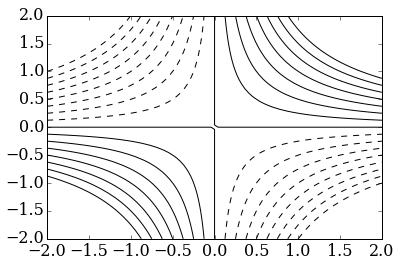
\includegraphics[width=0.5\textwidth]{clase06/m_1.png}
\caption{Líneas de flujo para $m=1$}
\label{fig:m_1}
\end{figure}
%
\begin{figure}
\centering
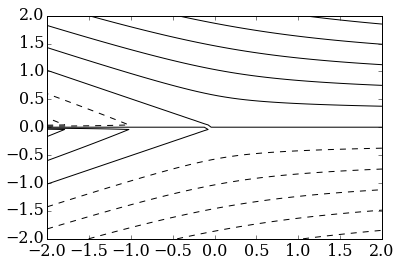
\includegraphics[width=0.5\textwidth]{clase06/m_01.png}
\caption{Líneas de flujo para $m=0.17$}
\label{fig:m_01}
\end{figure}
%
\begin{figure}
\centering
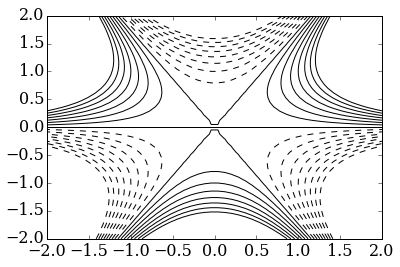
\includegraphics[width=0.5\textwidth]{clase06/m_2.png}
\caption{Líneas de flujo para $m=2$}
\label{fig:m_2}
\end{figure}

\section*{Espesor de capa límite de Falkner-Skan}
Usando el mismo método de resolución que en el caso de Blasius de la clase pasada, podemos resolver la Ec. \eqref{eq:F-S} numéricamente, y así obtener el valor del espesor de la capa límite.\footnote{\url{https://github.com/cdcooper84/mec220/blob/master/apuntes/clase06/falkner-skan.ipynb}}
Como es de imaginarse, este espesor depende de $m$.
Veamos dos casos: flujo contra una pared y sobre una cuña.

\paragraph*{Flujo contra una pared: $m=1$.}
Usando prueba y error, llegamos a que la condición de contorno $f''(0)$ tal que la condición $f'(\infty)=1$, es $f''(0)=0.871572$.
Así, resolvimos la ecuación diferencial y vimos que $f'(\eta) = 0.99$ en $\eta=3.37$. 
Considerando que en ese punto, $y=\delta$, podemos reeplazar en la Ec. \eqref{eq:eta_F-S} para llegar a
%
\begin{equation}
\frac{\delta}{x}=\frac{3.37}{\left((m+1)\frac{U_\infty x}{\nu}\right)^{1/2}} = \frac{3.37}{\sqrt{2\cdot Re_x}} 
\end{equation}

\paragraph*{Flujo sobre una cuña: $m=0.17$.}
En este caso, la condición de contorno correcta fue $f''(0)=0.547838$, y llegamos a que $f'(\eta)=0.99$ ocurre en $\eta=4.2$, por lo tanto, 
%
\begin{equation}
\frac{\delta}{x}=\frac{4.2}{\left((m+1)\frac{U_\infty x}{\nu}\right)^{1/2}} = \frac{3.37}{\sqrt{1.176\cdot Re_x}} 
\end{equation}

\section*{Capa límite con succión y soplido}
Entre las técnicas más recurrentes para el control de la capa límite está la succión y soplido. De hecho, la succión se usa en aplicaciones aerodinámicas para evitar la separación del flujo, lo que no solo disminuye la posibilidad de "stall", pero además reduce el arrastre sobre el cuerpo.

Para forzar la succión o soplido de la pared, podemos considerar una velocidad vertical $v_w$ en la pared, lo que cambia las condiciones de contorno de la ecuación de Blasius. Vimos en una clase reciente que la velocidad $v$ es
%
\begin{equation}
v = -\frac{U_\infty}{2}\left(\frac{\nu}{U_\infty x}\right)^{1/2}(f-f'\eta)
\end{equation}
%
pero en la pared, $v=v_w$, $\eta=0$ y $f'(0)=0$, y queda
%
\begin{equation}
\frac{v_w}{U_\infty} = -\frac{1}{2}\left(\frac{\nu}{U_\infty x}\right)^{1/2}f(0)
\end{equation}
%
lo que nos da una nueva condición de contorno para $f(0)$:
%
\begin{equation}
f(0) = -2\sqrt{Re_x}\frac{v_w}{U_\infty}
\end{equation}
%
Así, quedamos con la ecuación de Blasius:
%
\begin{equation}
f'''+\frac{1}{2}ff''=0
\end{equation}
%
donde sabemos que
%
\begin{align}
f'(\eta) = \frac{u}{U_\infty}\\
\eta = y\left(\frac{U_\infty}{\nu x}\right)^{1/2}
\end{align}
%
y las condiciones de borde
%
\begin{align}
f'(0) &= 0\\
f'(\infty) &= 1\\
f(0) &= -2\sqrt{Re_x}\frac{v_w}{U_\infty}=-2v_w^*
\end{align}

\paragraph*{Espesor de capa límite con soplido $v_w=0.1$.}
Resolviendo la ecuación de Blasius numéricamente\footnote{\url{https://github.com/cdcooper84/mec220/blob/master/apuntes/clase06/succion.ipynb}} con la condición de contorno modificada para $f(0)$, y la condición de contorno $f''(0)=0.2615$ para que se cumpla que $f'(\infty)=1$, nos damos cuenta que $u=0.99U_\infty$ en $\eta=5.32$. 
Como era de esperar, el soplido ensancha la capa límite (comparado con Blasius, donde $\eta=4.92$). De esta forma, podemos llegar a 
%
\begin{equation}
\frac{\delta}{x}=\frac{5.32}{\left(\frac{U_\infty x}{\nu}\right)^{1/2}} = \frac{5.32}{\sqrt{Re_x}} 
\end{equation}

\paragraph*{Espesor de capa límite con succión $v_w=-0.1$.}
En este caso, necesitamos setear $f''(0) = 0.4061$ para cumplir con la condición de contorno al infinito.
Numéricamente,\footnote{\url{https://github.com/cdcooper84/mec220/blob/master/apuntes/clase06/succion.ipynb}} nos damos cuenta que $u=0.99U_\infty$ para $\eta=4.58$. Como es de esperar, la succión adelgaza la capa límite, y llegamos a que
%
\begin{equation}
\frac{\delta}{x}=\frac{4.58}{\left(\frac{U_\infty x}{\nu}\right)^{1/2}} = \frac{4.58}{\sqrt{Re_x}} 
\end{equation}
